\documentclass[tikz,border=8pt]{standalone}
% Shared look for every TikZ diagram. Load with \input{../../tools/tikz-style.tex}
\usepackage[T1]{fontenc}
\usepackage{lmodern}
\renewcommand{\sfdefault}{lmr}  % diagrams use the same serif as the text
\usetikzlibrary{arrows.meta, positioning, shapes.geometric, calc, fit, backgrounds}
\definecolor{cblue}{HTML}{4C78A8}
\definecolor{corange}{HTML}{F58518}
\definecolor{cgreen}{HTML}{54A24B}
\definecolor{cred}{HTML}{E45756}
\definecolor{cpurple}{HTML}{B279A2}
\definecolor{cgrey}{HTML}{6B6B6B}
\tikzset{
  every picture/.style={font=\sffamily, line width=1.2pt},
  box/.style={draw=#1, fill=#1!12, rounded corners=4pt, align=center, inner sep=7pt, minimum height=1.1cm},
  box/.default=cgrey,
  arrow/.style={-{Stealth[length=3mm]}, draw=cgrey, line width=1.4pt},
  title/.style={font=\sffamily\bfseries\Large},
  note/.style={font=\sffamily\small, text=cgrey, align=center},
}
\AtBeginDocument{\hyphenpenalty=10000 \exhyphenpenalty=10000}

% Dynamic Bayes network of a robot: hidden states x_t in a chain, each made by the previous state and the command
% u_t; each reading z_t made by the current state only. Shaded nodes are known to the robot, white ones are hidden.
\begin{document}
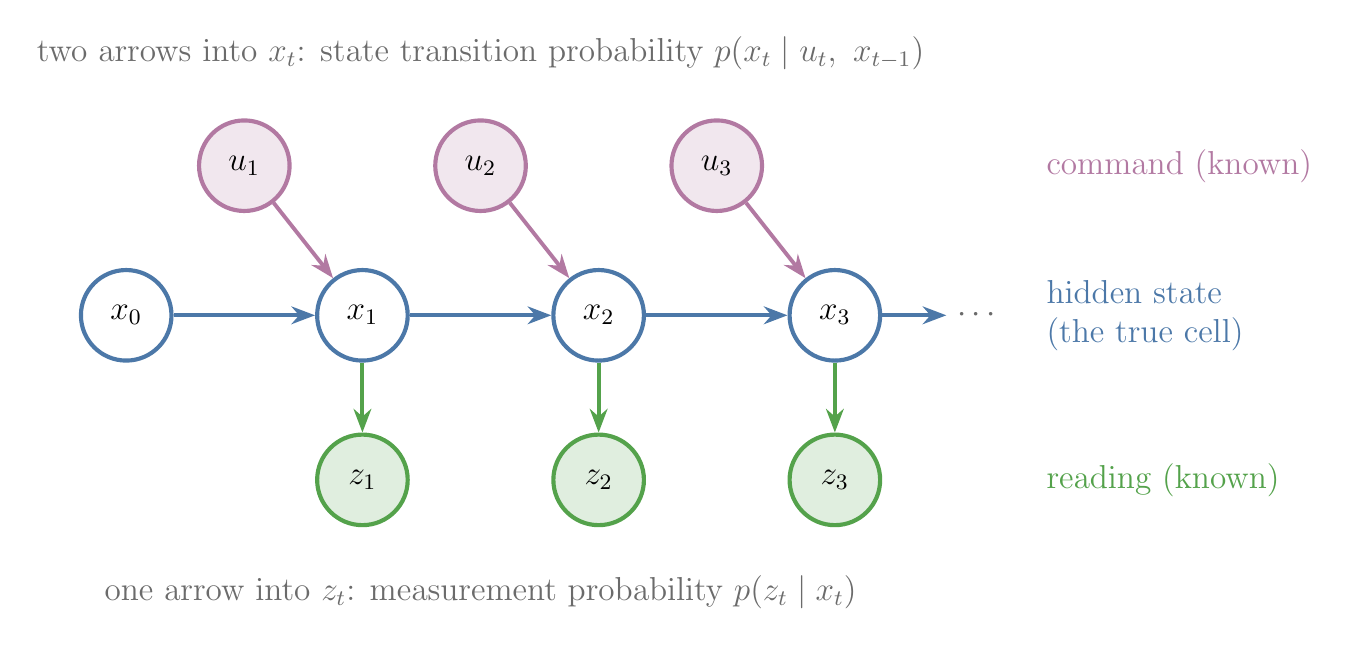
\begin{tikzpicture}[x=3cm, y=1.9cm, every node/.append style={font=\large},
    hid/.style={circle, draw=cblue, line width=1.5pt, minimum size=1.15cm, fill=white},
    obs/.style={circle, draw=#1, line width=1.5pt, minimum size=1.15cm, fill=#1!18}]
  \node[hid] (x0) at (0,0) {$x_0$};
  \foreach \t in {1,2,3} {
    \node[hid] (x\t) at (\t,0) {$x_\t$};
    \node[obs=cpurple] (u\t) at (\t-0.5,1) {$u_\t$};
    \node[obs=cgreen] (z\t) at (\t,-1.1) {$z_\t$};
    \draw[arrow, draw=cgreen] (x\t) -- (z\t);
    \draw[arrow, draw=cpurple] (u\t) -- (x\t);
  }
  \draw[arrow, draw=cblue] (x0) -- (x1);
  \draw[arrow, draw=cblue] (x1) -- (x2);
  \draw[arrow, draw=cblue] (x2) -- (x3);
  \node[cgrey] (dots) at (3.6,0) {$\cdots$};
  \draw[arrow, draw=cblue] (x3) -- (dots);
  % legends
  \node[anchor=west, cblue, align=left] at (3.85,0.0) {hidden state\\(the true cell)};
  \node[anchor=west, cpurple, align=left] at (3.85,1.0) {command (known)};
  \node[anchor=west, cgreen, align=left] at (3.85,-1.1) {reading (known)};
  \node[cgrey, align=center] at (1.5,1.75) {two arrows into $x_t$: state transition probability $p(x_t \mid u_t,\ x_{t-1})$};
  \node[cgrey, align=center] at (1.5,-1.85) {one arrow into $z_t$: measurement probability $p(z_t \mid x_t)$};
\end{tikzpicture}
\end{document}
